\begin{problem}{Impact on Polaris Deep}{standard input}{standard output}{2 seconds}{256 megabytes}

The research outpost \textit{Polaris Deep} orbits a dying star, and its only protection from the heat is a coolant network laid out on a grid of $n \times m$ tiles. Each tile is either empty or holds a junction. A junction has openings in two, three, or four of the four cardinal directions --- up, right, down, left. A junction with exactly one opening is physically impossible: the pressure would burst it instantly.

Two junctions in orthogonally adjacent tiles are \emph{connected} if and only if both have openings facing each other. A \emph{loop} is a route that starts at some junction, moves along connections, and returns to the starting junction without using any connection twice.

The chief engineer measures the network's resilience by the number of \emph{independent loops}$^{\dagger}$ it contains.

Each tile is described by a single integer $g_{i,j}$: $0$ for an empty tile, and otherwise the sum of $1$ for an opening facing up, $2$ for right, $4$ for down, and $8$ for left. For instance, a junction whose openings face up and right is written as $g_{i,j} = 1 + 2 = 3$:

\begin{center}
  \def \htmlPixelsInCm {45}
  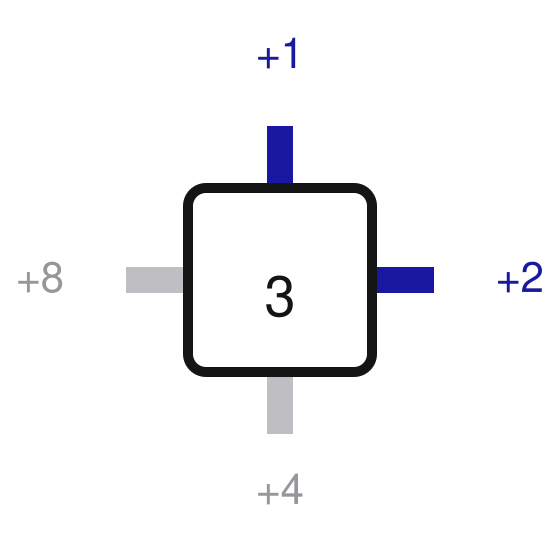
\includegraphics[width=3cm]{pipe-bits.svg}
\end{center}

Openings facing outside the grid connect to nothing.

During a micrometeorite storm the junctions are destroyed one by one. Telemetry predicts the whole sequence of $q$ impacts in advance: every impact hits a tile containing a working junction, and no tile is hit twice.

After each impact, report the number of independent loops remaining in the network.

{\small $^{\dagger}$ Formally, the \emph{number of independent loops} of the network is the largest $t$ for which one can choose a sequence of loops $L_1, L_2, \ldots, L_t$ such that every loop $L_i$ passes through at least one connection that none of the earlier loops $L_1, L_2, \ldots, L_{i-1}$ pass through.}


\InputFile
The first line contains a single integer $t$ ($1 \le t \le 2 \cdot 10^5$) --- the number of test cases.

The first line of each test case contains two integers $n$ and $m$ ($1 \le n, m$, $n \cdot m \le 2 \cdot 10^5$) --- the dimensions of the grid.

Each of the next $n$ lines contains $m$ integers $g_{i,1}, g_{i,2}, \ldots, g_{i,m}$ ($0 \le g_{i,j} \le 15$) --- the tiles of the $i$-th row, encoded as described in the statement, rows listed from top to bottom.

The next line contains a single integer $q$ ($0 \le q$) --- the number of impacts.

Each of the next $q$ lines contains two integers $r$ and $c$ ($1 \le r \le n$, $1 \le c \le m$) --- the tile destroyed by the next impact.

It is guaranteed that no tile is hit twice, that every impacted tile contains a junction, that $q$ does not exceed the number of junctions, and that the sum of $n \cdot m$ over all test cases does not exceed $2 \cdot 10^5$.


\OutputFile
For each test case, print a single line containing $q$ integers: the $i$-th integer must be the number of independent loops remaining after the first $i$ impacts.

If $q = 0$, print an empty line.


\Example

\begin{example}
\exmpfile{example.01}{example.01.a}%
\end{example}

\Note
In the first test case every tile holds a $4$-opening junction, giving two independent loops (the two unit squares). Destroying tile $(1,1)$ breaks the left one and destroying tile $(1,2)$ breaks the other, hence $1\ 0\ 0$. In the second test case the eight outer junctions form a single loop around the centre, while the centre tile is connected to nothing, so removing it first changes nothing: $1\ 0$. In the third test case there are no connections at all, and in the fourth $q = 0$, so the answer line is empty.


\end{problem}

